\documentclass[11pt]{article}
\usepackage{graphicx} %for displaying images
\usepackage{float}
\usepackage{listings}
\usepackage{color}


\definecolor{dkgreen}{rgb}{0,0.6,0}
\definecolor{gray}{rgb}{0.5,0.5,0.5}
\definecolor{mauve}{rgb}{0.58,0,0.82}

\lstset{frame=tb,
	language=Python,
	aboveskip=3mm,
	belowskip=3mm,
	showstringspaces=false,
	columns=flexible,
	basicstyle={\small\ttfamily},
	numbers=none,
	numberstyle=\tiny\color{gray},
	keywordstyle=\color{blue},
	commentstyle=\color{dkgreen},
	stringstyle=\color{mauve},
	breaklines=true,
	breakatwhitespace=true,
	tabsize=3
}

%----------------------------------------------------------------------------------------
%	TITLE SECTION
%----------------------------------------------------------------------------------------
\title{	
	\normalfont\normalsize
	\textsc{Old Dominion University}\\ % Your university, school and/or department name(s)
	\vspace{25pt} % Whitespace
	\rule{\linewidth}{0.5pt}\\ % Thin top horizontal rule
	\vspace{20pt} % Whitespace
	{\huge Assignment Four}\\ % The assignment title
	\vspace{12pt} % Whitespace
	\rule{\linewidth}{2pt}\\ % Thick bottom horizontal rule
	\vspace{20pt} % Whitespace
}
\author{\LARGE Joshua Gahan} % Your name
\date{\normalsize\today} % Today's date (\today) or a custom date

\begin{document}
	\pagenumbering{gobble}
	\maketitle %render title
	\newpage
	\pagenumbering{arabic}
	
	\section{Twitter Follower comparison}
	\hspace{10mm} We enumerated Nwala's twitter profile and then gathered both his number of twitter followers. and the number of twitter followers that his followers had. We did this in order to see if the Friendship paradox holds for his twitter account
	\subsection{Retrieval of Twitter Follower data}
	\begin{lstlisting}
	try:
	    for follower in tweepy.Cursor(api.followers, screen_name="acnwala").items():
	        data.append(follower.screen_name)
	        print(follower.screen_name)
	        outFile.write("%s\n" % follower.screen_name)
	except Exception as e:
	    print(str(e))
	
	with open('data.txt', 'r') as inFile:
	    for entry in inFile:
	        with urllib.request.urlopen("https://twitter.com/%s" % entry.strip()) as res:
	            baseHMTL = res.read()
	            soup = BeautifulSoup(baseHMTL, features="html.parser")
	
	            tags = soup.findAll("span", class_="ProfileNav-value")
	            followers = tags[2]
	            try:
	               followers = followers["data-count"]
	               with open('follow_data', 'a') as finalFile:
	                  print("%s, %d" % (entry.strip(), int(followers)))
	                  finalFile.write("%s, %d\n" % (entry.strip(), int(followers)))
	               except KeyError:
	                  with open('follow_data', 'a') as finalFile:
	                     finalFile.write("%s, %d\n" % (entry.strip(), 0))
	\end{lstlisting}
	\hspace{10mm} We used tweepy to extract the names of our followers. For each follower, we then issued a http request to the follower's twitter profile, and then used Beautiful soup to strip the follower count out of the received HTML. Twitter stores the relevant values in spans with the class "ProfileNav-value," of which the second (tag[2]) represents the follower count. Within this second retrieved span the "data-count" member contains the follower count. 
	\section{Facebook Friend Comparison}
	\hspace{10mm} Using the provided data for Nwala's 2014 Facebook account, we read in and sorted the data in this list. This was used for plotting later. 
	\section{Findings}
	\hspace{10mm} We found upon plotting our data that the Friendship Paradox holds for both his twitter and his Facebook profiles. His 250 twitter followers was below the median and mean count of the number of followers his followers had. This held true for Facebook as well, with his ninety-eight Facebook friends being well below the median and mean values for our data. Our findings our represented in the below graphs. 
	\begin{figure}[h!]
		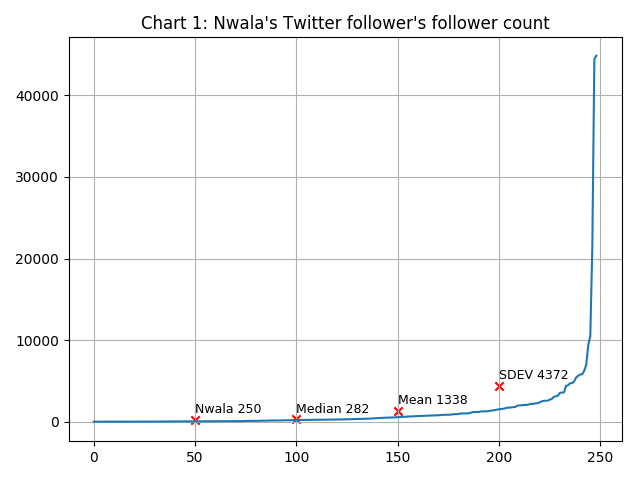
\includegraphics[scale=0.5]{resources/twitter_followers.png}
		\caption{Nwala's Twitter Follower's followers}
	\end{figure}
	\begin{figure}[h!]
		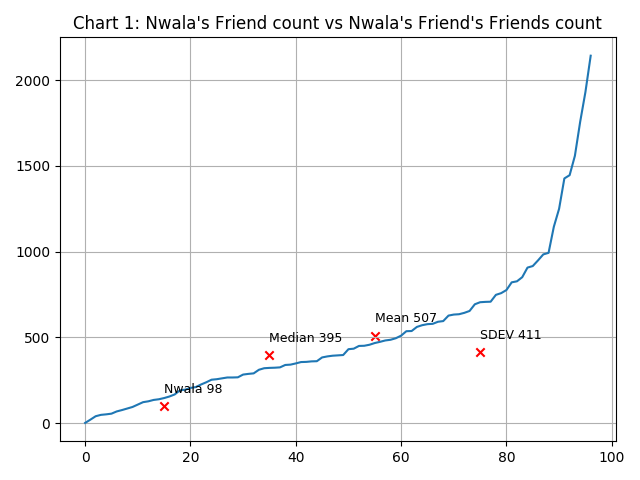
\includegraphics[scale=0.5]{resources/fb.png}
		\caption{Number of friends that Nwala's Facebook friends have vs him.}
	\end{figure}
	

\end{document}